\documentclass[18pt]{beamer}
\usepackage[utf8]{inputenc} % for the umlauts
\usepackage{subfigure}

\beamertemplatenavigationsymbolsempty
%% SLIDE FORMAT

% use 'beamerthemekit' for standard 4:3 ratio
% for widescreen slides (16:9), use 'beamerthemekitwide'

\usepackage{templates/beamerthemekit}
% \usepackage{templates/beamerthemekitwide}

\setcounter{tocdepth}{1}

%% TITLE PICTURE

% if a custom picture is to be used on the title page, copy it into the 'logos'
% directory, in the line below, replace 'mypicture' with the 
% filename (without extension) and uncomment the following line
% (picture proportions: 63 : 20 for standard, 169 : 40 for wide
% *.eps format if you use latex+dvips+ps2pdf, 
% *.jpg/*.png/*.pdf if you use pdflatex)

%\titleimage{mypicture}

%% TikZ INTEGRATION

\usepackage{tikz-uml}
% use these packages for PCM symbols and UML classes
% \usepackage{templates/tikzkit}
 \usepackage{templates/tikzuml}

% the presentation starts here
\usepackage{csquotes}

\usepackage{mathabx}
\usepackage{picture}
\usepackage[absolute,overlay]{textpos}
%\usepackage[texcoord,grid,gridunit=mm,gridcolor=red, subgridcolor=green]{eso-pic}
\setbeamercovered{invisible}
\setbeamertemplate{caption}{\raggedright\insertcaption\par}


\title[SWT1]{Softwaretechnik 1 - 2. Tutorium}
\subtitle{Tutorium 17}
\author{Felix Bachmann}
\date{28.05.2019}

\institute{KIT - Institut für Programmstrukturen und Datenorganisation (IPD)}

\usetikzlibrary{positioning}

\begin{document}

% change the following line to "ngerman" for German style date and logos
\selectlanguage{ngerman}

%title page
\begin{frame}
\titlepage
\end{frame}

\section{Orga}
\begin{frame}[fragile]{Abgabemodalitäten}
	\begin{block}{Sprache}
		\begin{itemize}
			\item letztes Mal kam eine Frage, ob Abgaben auf Englisch auch erlaubt
			\item für mich ok
			\item laut Übungsleitern in Klausur nicht ok
			\begin{itemize}
				\item also am besten jetzt auch schon auf Deutsch abgeben
			\end{itemize}
		\end{itemize}
	\end{block}
	\begin{block}{Notation Abstrakte Klassen}
		\begin{itemize}
			\item an VL-Notation halten (insbesondere nicht \verb|<<abstract>>|)
			\item siehe UML-Spec 
			\begin{itemize}
				\item \url{https://www.omg.org/spec/UML/2.5.1/PDF}, p.101
			\end{itemize}
		\end{itemize}
	\end{block}
\end{frame}

\begin{frame}{Tutorientermine}
	\begin{itemize}
		\item entsprechend der Abstimmung vom vorletzten Mal ist das nächste Tut am 04.06 (= nächste Woche)
		\item also
		\begin{itemize}
			\item 28.05. (heute): Tutorium
			\item 04.06.: Tutorium
			\item 11.06.: kein Tutorium
			\item 18.06.: kein Tutorium
			\item ab 25.06. wieder regulär 14-tägig
			\begin{itemize}
				\item 25.06, 09.07, 23.07
			\end{itemize}
		\end{itemize}
	\end{itemize}
\end{frame}

\subsection{Feedback 2. Übungsblatt}
\begin{frame}
	\frametitle{2. Übungsblatt Statistik}
	\includegraphics[scale=0.7]{./pics/tut2/statistics-ub2.png}
\end{frame}
	
\subsection{2. Übungsblatt - Fehler (Allgemein)}
\begin{frame}
		\frametitle{Häufige Fehler}
		\begin{block}{Allgemein}
			\includegraphics[scale=0.6]{./pics/tut2/deckblatt.png}
			\begin{itemize}
				\item $\implies$ nur das offizielle Deckblatt verwenden!
				\pause
				\item häufigster Fehler: Aufgaben nicht abgegeben
			\end{itemize}
		\end{block}
\end{frame}
	
\subsection{2. Übungsblatt - Fehler}
\begin{frame}
		\frametitle{Häufige Fehler}
		\begin{block}{Aufgabe 1 (Lastenheft)}
			\begin{itemize}
				\item \enquote{relevante Daten} bei Produktdaten ist unpräzise
				\pause
				\item Verwirrung: Szenario vs. \enquote{Aufgaben-Szenario}
				\pause
				\item Anwendungsfalldiagramm
				\begin{itemize}
					\item Syntax (Pfeile, System-Kasten, Aktoren,\dots)
					\item Anwendungsfälle enthalten Verben
					\begin{itemize}
						\item \enquote{Vorschau}, \enquote{Kundenbilder} sind \textbf{keine}
						\item richtig wäre z.B. \enquote{Kundenbilder speichern}
					\end{itemize}
					\item direkte Verbindungen zwischen Anwendungsfällen nicht definiert
					\begin{itemize}
						\item include vs. extend
						\item auch nicht zwischen Aktoren
					\end{itemize}
				\end{itemize}
			\end{itemize}
		\end{block}
\end{frame}

\begin{frame}
		\frametitle{Häufige Fehler}
		\begin{block}{Aufgabe 2 (Klassendiagramm)}
			\begin{itemize}
				\item äußere Form, UML-Syntax
				\begin{itemize}
					\item gerichtete Assoziation vs. Vererbung
					\item $\underbrace{\texttt{name:Typ}}_{\text{UML}}$ statt $\underbrace{\texttt{Typ name}}_{\text{Java}}$
				\end{itemize}
				\pause
				\item alle Klassen, die ihr verwendet, müssen auch im Diagramm sein
				\begin{itemize}
					\item z.B. \enquote{Bild} als Parameter verwendet, aber nirgendwo definiert
				\end{itemize}
				\pause
				\item \texttt{verarbeite(b:Bild):Bild} in Einzelbildop./Mehrbildop. nicht als abstrakt gekennzeichnet
				\begin{itemize}
					\item kann man aber nicht sinnvoll implementieren
				\end{itemize}
				\pause
				\item Farbtiefe sollte Enum sein (nur bestimmte Werte erlaubt)
				\pause
				\item oft wurden die konkreten Operationen als Methoden hingeschrieben
				\begin{itemize}
					\item sollten aber eigene Klassen sein
					\item Wieso ist das sinnvoll? siehe \enquote{Befehl/Command}-Entwurfsmuster 
					\item (nächstes Tut)
				\end{itemize}
			\end{itemize}
		\end{block}
\end{frame}

\begin{frame}
\frametitle{Häufige Fehler}
\begin{block}{Aufgabe 2 (Klassendiagramm)}
	\begin{itemize}
		\item bei Collections immer []-Schreibweise nutzen, nicht \texttt{ArrayList<XY>}
		\pause
		\item uses. vs Assoziation
	\end{itemize}
\end{block}
\pause
	\begin{block}{Aufgabe 3 (Durchführbarkeitsanalyse)}
	\begin{itemize}
		\item nur Stichpunkte\dots
		\pause
		\item Fragen beantworten, nicht stellen!
		\linebreak z.B. "'Es werden 3 Java-Entwickler benötigt."' $\implies$
		"'Da wir 5 zur Zeit untätige Java-Entwickler in der Firma haben, ist das Projekt aus personeller Sicht für die Pear Corp. durchführbar."'
	\end{itemize}
\end{block}
\end{frame}

\begin{frame}
		\frametitle{Häufige Fehler}
		\begin{block}{Aufgabe 4 (HDR programmieren)}
			\begin{itemize}
				\item Überprüfungen bei Matrix-Operationen vergessen
				\begin{itemize}
					\item \texttt{A*B} nur möglich, wenn \texttt{A.cols() == B.rows()}
					\item \texttt{$A^{-1}$} nicht-existent falls \texttt{A} nicht quadratisch
					\begin{itemize}
						\item existiert nur, falls \texttt{det(A) != 0}
					\end{itemize}
				\end{itemize}
				\pause
				\item die \enquote{komplizierteren} Sachen nicht abgegeben
				\begin{itemize}
					\item keine Angst vor ein bisschen Mathe :)
				\end{itemize}
				\pause
				\item zu wenig oder nicht sinnvoll getestet
				\pause
				\item Überraschung: \texttt{mtx.copy()} soll Matrix kopieren
			\end{itemize}
		\end{block}
	

\end{frame}

\begin{frame}{Häufige Fehler}
	\begin{block}{Aufgabe 5 (Kommandozeilen-Tool)}
	\begin{itemize}
		\item 5 Abgaben \dots
		\item kleine Fehler in pom (dependencies kopieren)
	\end{itemize}
\end{block}

\pause

\begin{block}{Aufgabe 6 (Filter-Schnittstellen)}
	\begin{itemize}
		\item 4 Abgaben \dots
		\item Filter-Liste sollte veränderbar sein
		\begin{itemize}
			\item z.B. Pipeline-Muster
		\end{itemize}
	\end{itemize}
\end{block}
\end{frame}


\section{Substitutionsprinzip}
\begin{frame}{Liskov'sches Substitutionsprinzip}
	\small aka Verhaltenskonformanz, Klientencode-Wiederverwendung
	\begin{block}{Definition}
		In einem Programm, in dem U eine Unterklasse
		von O ist, kann jedes Exemplar der Klasse O
		durch ein Exemplar von U ersetzt werden, wobei
		das Programm weiterhin korrekt funktioniert.
	\end{block}
	\pause
	\begin{itemize}
		\item aus Sicht des Verhaltens ist jedes U-Objekt auch ein O-Objekt
		\item Klientencode muss bei Methodenaufrufen nicht wissen, ob es sich um ein U-Objekt oder O-Objekt handelt
	\end{itemize}
	\pause
	\begin{alertblock}{Achtung}
		Das müssen wir als Programmierer sicherstellen. Nur weil Java uns die Möglichkeit bietet Unterklassen zu bilden, ist das Substitutionsprinzip noch lange nicht erfüllt! (dadurch ist nur die sogenannte Typkonformanz gegeben)
	\end{alertblock}
\end{frame}

\begin{frame}{Liskov'sches Substitutionsprinzip}
	\huge \centering Beispiel!
\end{frame}

\section{Zustandsdiagramm}
	\subsection{Intro(1)}
	\begin{frame}
		\frametitle{Wo sind wir? Pflichtenheft!}
		\begin{enumerate}
			\item Zielbestimmung  
			\item Produkteinsatz 
			\item Produktumgebung
			\item Funktionale Anforderungen 
			\item Produktdaten 
			\item Nichtfunktionale Anforderungen 
			\item Globale Testfälle
			\item Systemmodelle
			\begin{itemize}
				\item Szenarien
				\item Anwendungsfälle
				\item Objektmodelle $\implies$ UML-Klassendiagramme (letztes mal)
				\item \underline{\textbf{Dynamische Modelle}}
				\begin{itemize}
					\item UML-Zustandsdiagramm
					\item UML-Aktivitätsdiagramm
					\item UML-Sequenzdiagramm
					\makebox(0,0){\put(0,3.3\normalbaselineskip){%
							$\left.\rule{0pt}{1.5\normalbaselineskip}\right\}$ Heute!}}
				\end{itemize}
				\item Benutzerschnittstelle$\implies$ Zeichnungen/Screenshots
			\end{itemize}
			\item Glossar 
		\end{enumerate}
	\end{frame}

	\subsection{Intro(2)}
	\begin{frame}
		\frametitle{Begriffsklärung}
		\includegraphics[scale=0.35]{./pics/tut1/uml_diagrams.png}
	\end{frame}

	\subsection{ZD: Allgemein}
	\begin{frame}
		\frametitle{Zustandsdiagramm \\ - Mein Entwurf bekommt Zustände}
		\begin{block}{Wozu braucht man das?}
			\pause
			\begin{itemize}
				\item Zustand \textbf{eines Objektes} beschreiben
				\item Zustandsüberführungsfunktion?
			\end{itemize}
		\end{block}
	\end{frame}

	\subsection{ZD: Allgemein (2)}
	\begin{frame}
		\frametitle{Zustandsdiagramm $\approx$ endlicher Automat}
		\begin{figure}
			\subfigure[GBI: DEA]{\includegraphics[scale=0.23]{./pics/tut2/auto_gbi.png}}
			\subfigure[SWT: Zustandsdiagramm]{\includegraphics[scale=0.2]{./pics/tut2/auto_swt.png}}
		\end{figure}
	\end{frame}
	
	\begin{frame}{Zustände}
		\begin{figure}
			\centering
			\begin{tikzpicture}
				\begin{umlstate}[x=0, y=0, name=state, rectangle split parts=0, entry=\texttt{methodCalledOnEntry()}, exit=\texttt{methodCalledOnExit()}]{ZustandsName} \end{umlstate}
			\end{tikzpicture}
		\end{figure}
		\begin{itemize}
			\item es können Methoden angegeben werden, die ausgeführt werden bei
			\begin{itemize}
				\item Übergang in den Zustand hinein (entry)
				\item Übergäng aus dem Zustand heraus (exit)
			\end{itemize}
			\item falls kein entry und exit, kann man Unterteilung auch weglassen
		\end{itemize}
	\end{frame}

\begin{frame}{Zustandsübergänge}
	\begin{figure}
		\centering
			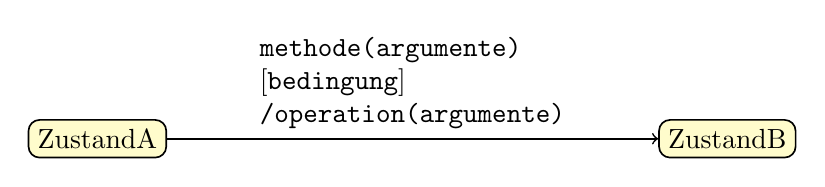
\begin{tikzpicture}[stateNode/.style={rectangle, draw, rounded corners, fill=yellow!20}, semithick]
		\node[stateNode, draw] at (0,0) (a) {ZustandA};
		\node[stateNode, draw] at (8,0) (b) {ZustandB};
		\draw[->] (a) node[above, align=left, xshift=4cm] { \texttt{methode(argumente)} \\ \lbrack \texttt{bedingung}\rbrack \\ \texttt{/operation(argumente)}} -- (b);
		\end{tikzpicture}
	\end{figure}

	\begin{itemize}
		\item Übergang von ZustandA nach ZustandB findet statt, wenn
		\begin{itemize}
			\item in ZustandA \texttt{methode(argumente)} ausgeführt wird, und
			\item \lbrack \texttt{bedingung}\rbrack~gilt
		\end{itemize} \pause
		\item \texttt{methode(argumente)} ist optional, $\epsilon$-Übergänge sind möglich
		\item  \lbrack \texttt{bedingung}\rbrack~ebenfalls optional
		\item  \texttt{/operation(argumente)} wird bei Übergang ausgeführt
		\begin{itemize}
			\item ist auch optional
		\end{itemize} \pause
		\item auch reflexive Übergänge möglich
	\end{itemize}
\end{frame}

\begin{frame}{Mögliche Übergänge}
	(Tafel)
\end{frame}

\begin{frame}{Start- und Endzustand}
		\begin{figure}
		\centering
		\begin{tikzpicture}[stateNode/.style={rectangle, draw, rounded corners, fill=yellow!20}, semithick]
			\node[stateNode, draw] at (4,0) (a) {ZustandA};
			\node[stateNode, draw] at (8,0) (b) {ZustandB};
			\node[] at (9.9, 0) (help) {};
			\draw[->] (a) -- (b);
			
			\umlstateinitial[x=0, y=0,name=init, width=2ex]
			
			\umlstatefinal[x=10, y=0,name=final, width=2ex]
			
			\draw[->] (init) -- (a);
			\draw[->] (b) -- (help);
		\end{tikzpicture}
	\end{figure}
	\begin{itemize}
		\item Startzustand muss immer da sein
		\item Endzustand ist optional
	\end{itemize}
\end{frame}

\begin{frame}{Beispiel}
	\centering
	\begin{tikzpicture}[stateNode/.style={rectangle, draw, rounded corners, fill=yellow!20}, semithick]
		\begin{umlstate}[x=0, y=5, name=m, entry=\texttt{gähnen()}]{müde} \end{umlstate}
		\begin{umlstate}[x=8, y=5, name=s, entry=\texttt{entspannen()}]{schlafend} \end{umlstate}
		\node[stateNode, draw] at (4, 9) (w) {hellwach};
		\draw[->] (w.west) node[above, xshift=-2cm] { \lbrack \texttt{wachInStunden >= 14}\rbrack} -| (m.north);
		\draw[->] (m.east) node[above, xshift=2cm] {\texttt{augenZu()}} -- (s.west);
		
		\draw[->] (s) node[above, align=center, yshift=3.35cm, xshift=-1.5cm] {\texttt{weckerKlingelt()} \\ \texttt{/weckerAus()}} |- (w);
		
		\umlstateinitial[x=4, y=10,name=init, width=2ex]
		\draw[->] (init) -- (w);
		
		\node[above right=1cm and -2.1cm of s](help-1) {};
		\draw[-] (s.80) -- (help-1.center);
		\draw[->] (help-1.center) node[above,xshift=0.9cm, align=center] {\footnotesize \texttt{schnarchen()}} -| (s.30);
	\end{tikzpicture}
	\pause
	\begin{itemize}
		\item Achtung, reflexive Übergänge führen auch entry und exit aus!
		\begin{itemize}
			\item \texttt{entspannen()} wird ggf. mehrfach aufgerufen
		\end{itemize}
	\end{itemize}
\end{frame}

	\subsection{ZD: Syntax(1)}
	\begin{frame}
		\frametitle{Zustandsdiagramm: Syntax}
		\begin{figure}
			\includegraphics[scale=0.4]{./pics/tut2/auto_swt.png}
		\end{figure}	
	\end{frame}

	\subsection{ZD: Syntax (2)}
	\begin{frame}
		\frametitle{Zustandsdiagramm: Hierarchie}
		\includegraphics[scale=0.7]{./pics/tut2/auto_hier.png}	
		\begin{itemize}
			\item nicht mächtiger, aber übersichtlicher
		\end{itemize}
	\end{frame}

	\subsection{ZD: Syntax (3)}
	\begin{frame}
		\frametitle{Zustandsdiagramm: Hierarchie - History}
		\begin{itemize}
			\item  History-Element, damit sich Hierarchie den letzten Zustand merkt
		\end{itemize}
		\includegraphics[scale=0.5]{./pics/tut2/auto_hier-hist.png}
		\pause	
		\begin{itemize}
			\item a, c, d $\implies$ C (ohne History wäre es A)
		\end{itemize}
	\end{frame}

	\subsection{ZD: Syntax(4)}
	\begin{frame}
		\frametitle{Zustandsdiagramm: Nebenläufigkeit}	
		\begin{itemize}
			\item  mehrere Zustandsdiagramme in einem
		\end{itemize}
		\centering
		\includegraphics[scale=0.5]{./pics/tut2/auto_par.png}	
		\begin{itemize}
			\item Zustand angegeben durch Kombination aus Zuständen
			\begin{itemize}
				\item z.B. AxC, BxC, \dots
			\end{itemize} 
		\end{itemize}
	\end{frame}

	\subsection{ZD: Aufgabe}
	\begin{frame}
		\frametitle{Klausuraufgabe SS09}
		\begin{block}{Aufgabe}
			Gegeben ist der folgende UML-Zustandsautomat. Geben Sie an, in welcher Zustandskombination
			sich der Zustandsautomat, jeweils ausgehend vom Startzustand, nach den beiden Eingabefolgen
			befindet.
		\end{block}
		\centering
		\includegraphics[scale=0.7]{./pics/tut2/auto_ex.png}
		\begin{itemize}
			\item 1. Eingabefolge: a, b, c, c \pause $\implies$ AxD
			\item 2. Eingabefolge: c, c, a, b, b, a, c, c, a \pause $\implies$ BxC
		\end{itemize}
	\end{frame}

	\begin{frame}{Klausuraufgabe SS09 (verkürzt)}
	\begin{block}{Szenario}
	\small	Zu Beginn wartet der Automat auf die Auswahl des Produktes durch den Kunden. Die
		Produktauswahl findet in zwei Schritten statt. Zunächst wählt der Kunde die Ebene, in
		welcher sich das gewünschte Produkt befindet. Wählt der Kunde eine Ebene aus, die
		nicht existiert, wartet der Automat weiter auf die Produktauswahl. Ist die Ebene gewählt,
		gibt der Kunde das Fach des gewünschten Produktes an. Nach der Produktauswahl wirft der Kunde so lange
		Münzen ein, bis der eingeworfene Betrag gleich oder größer dem Preis des ausgewählten
		Produktes ist. Solange der Kunde nicht ausreichend Geld in den Automaten eingeworfen
		hat, wartet der Automat auf den Einwurf des fehlenden Geldbetrages. Hat der
		Kunde ausreichend Geld eingeworfen, befördert der Automat das gewählte Produkt in
		den Ausgabeschacht. Danach entnimmt der Kunde das Produkt und der Automat wartet auf die nächste Produktauswahl.
	\end{block}
		Modellieren Sie das Verhalten des Automaten wie im obigen Szenario beschrieben als UML-Zustandsdiagramm.
		Geben Sie zu jedem Übergang das auslösende Ereignis sowie ggf. die
		notwendigen Bedingungen an.
\end{frame}
		
\section{Aktivitätsdiagramm}
	\subsection{AD: Allgemein(1)}
	\begin{frame}
		\frametitle{Aktivitätsdiagramm - Allgemein}
		\begin{block}{Wozu braucht man das?}
			\pause
			\begin{itemize}
				\item Ablaufbeschreibungen (Kontrollfluss, Objektfluss)
				\item i.A. \textbf{mehrere verschiedene} Objekte
			\end{itemize}
		\end{block}
	\end{frame}

	\subsection{AD: Allgemein(2)}
	\begin{frame}
		\frametitle{Aktivitätsdiagramm - Beispiel}
		\begin{itemize}
			\item ist ebenfalls nicht neues!
		\end{itemize}
		\centering
		\includegraphics[scale=0.35]{./pics/tut2/act_wat.png}
	\end{frame}

	\subsection{AD: Syntax(1)}
	\begin{frame}
		\frametitle{Aktivitätsdiagramm - Syntax}
		\includegraphics[scale=0.45]{./pics/tut2/act_syn1.png}
	\end{frame}

	\begin{frame}
	\frametitle{Aktivitätsdiagramm - Ablauf}
	\begin{itemize}
		\item Start am Startknoten mit einer Marke
		\item Aktionen werden erst ausgeführt, wenn an jedem Eingang eine Marke anliegt
		\item wurde eine Aktion ausgeführt, erscheinen an all ihren Ausgängen Marken
	\end{itemize}
	\end{frame}

	\subsection{AD: Syntax(2)}
	\begin{frame}
		\frametitle{Aktivitätsdiagramm - Syntax}
		\includegraphics[scale=0.45]{./pics/tut2/act_syn2.png}
	\end{frame}

	\subsection{AD: Syntax(3)}
	\begin{frame}
		\frametitle{Aktivitätsdiagramm - Syntax}
		\includegraphics[scale=0.45]{./pics/tut2/act_syn3.png}
	\end{frame}

	\subsection{AD: Beispiel}
	\begin{frame}
		\frametitle{Aktivitätsdiagramm - Beispiel}
		\begin{figure}
			\centering
			\caption{Wie kommt man hier zum Endknoten?}
			\includegraphics[scale=0.4]{./pics/tut2/act_ex.png}
		\end{figure}
	\end{frame}

	\begin{frame}{Noch ein Beispiel}
	 	(Tafel)
\end{frame}

	\begin{frame}{Klausuraufgabe SS 11}
	\begin{exampleblock}{Aufgabenstellung}
		Modellieren Sie das gegebene Szenario als UML-Aktivitätsdiagramm. Verwenden Sie bei Ihrer
		Modellierung korrekte UML-Notation. Objektflüsse müssen Sie nicht modellieren. 
	\end{exampleblock}
	(Szenario auf nächster Folie)
\end{frame}

\begin{frame}{Klausuraufgabe SS 11: Szenario}
\begin{block}{Szenario}
	\small Bernd Bruegge fühlt sich nicht wohl und möchte sich untersuchen lassen, um eine Diagnose zu erhalten. Er geht dazu ins Krankenhaus und meldet sich an der Pforte. Der
	Pförtner macht ihn darauf aufmerksam, dass er seine Krankenkassenkarte dabei haben
	muss – falls nicht, kann ihm keine Diagnose gestellt werden. Bernd B. hat seine Krankenkassenkarte dabei und lässt sich daher den Weg zur Patientenaufnahme zeigen, da
	er sich dort zunächst anmelden muss. Während der Sachbearbeiter an der Patientenaufnahme die Krankenakte mit den persönlichen Daten anlegt, füllt Bernd B. den
	Anamnesebogen aus. Danach wird Bernd B. vom Arzt untersucht. Die Untersuchung
	ergibt, dass der Arzt zur weiteren Diagnose ein Blutbild und ein Röntgenbild der Lunge
	benötigt und er in der Zwischenzeit ein Gespräch mit einem anderen Patienten führen
	kann. Dazu wird Bernd B. zunächst Blut abgenommen. Während das Blut im Labor
	analysiert wird, geht Bernd B. in die radiologische Abteilung und lässt das Röntgenbild
	der Lunge anfertigen. Als der Arzt von seinem Gespräch mit dem anderen Patienten zurückkommt, liegen das Röntgen- und das Blutbild vor und er stellt Bernd B. eine Diagnose.
\end{block}
\end{frame}

\begin{frame}
\frametitle{Musterlösung}
\centering
\includegraphics[scale=0.35]{./pics/tut2/solution-act.png}
\includegraphics[scale=0.4]{./pics/tut2/solution-act-points.png}
\end{frame}

\section{Sequenzdiagramm}
	\subsection{SD: Allgemein}
	\begin{frame}
		\frametitle{Sequenzdiagramm - Allgemein}
		\begin{block}{Wozu braucht man das?}
			\pause
			\begin{itemize}
				\item stellt den möglichen Ablauf eines Anwendungsfalls dar
				\item \textbf{zeitlicher Verlauf} von Methodenaufrufen, Objekterstellung, Objektzerstörung
			\end{itemize}
		\end{block}
	\end{frame}

	\subsection{SD: Syntax(1)}
	\begin{frame}
		\frametitle{Sequenzdiagramm - Syntax}
		\begin{itemize}
			\item Zeit verläuft von oben nach unten
			\item ein Kasten pro Objekt (\texttt{\underline{instanzName: KlassenName}})
			\item Lebenslinie
			\begin{itemize}
				\item gestrichelte senkrechte Linie
				\item eine pro Objekt, solange wie Objekt \enquote{lebt}
			\end{itemize}
			\item Steuerungsfokus
			\begin{itemize}
				\item dicker Balken über Lebenslinie
				\item zeigt, dass Objekt gerade aktiv ist
			\end{itemize}
			\item Nachrichtentypen (für Methodenaufrufe und Rückgabe)
			\begin{itemize}
				\item Synchrone Nachricht (blockierend)
				\item Antwort (optional)
				\item Asynchrone Nachricht
			\end{itemize}
			\begin{textblock*}{20mm}(75mm,63mm)
				\includegraphics[scale=0.4]{./pics/tut2/sd_met.png}
			\end{textblock*}
		\end{itemize}
	\end{frame}

	\subsection{SD: Syntax(2)}
	\begin{frame}
		\frametitle{Sequenzdiagramm - Syntax}
			\includegraphics[scale=0.4]{./pics/tut2/sd_ex.png}
	\end{frame}

	\subsection{SD: Syntax(2)}
	\begin{frame}
		\frametitle{Sequenzdiagramm - Syntax}
		\begin{figure}
			\centering
			\subfigure[Objekt-Erzeugung]{\includegraphics[scale=0.35]{./pics/tut2/sdcrea.png}}\newline
			\subfigure[Objekt-Zerstörung]{\includegraphics[scale=0.2]{./pics/tut2/sddestr.png}}
		\end{figure}
	\end{frame}

	\subsection{SD: Aufgabe}
	\begin{frame}
		\frametitle{Klausuraufgabe SS14}
			\begin{figure}
				\centering
				\includegraphics[scale=0.65]{./pics/tut2/sdtask.png}
				\caption{Hier stimmt was nicht\dots, aber was?}
			\end{figure}
	\end{frame}

\begin{frame}{Musterlösung 1}
	\includegraphics[scale=0.65]{pics/tut2/solution-seq.png}
\end{frame}

\begin{frame}{Musterlösung 2}
	\includegraphics[scale=0.65]{pics/tut2/solution-seq-l1.png}
\end{frame}

\begin{frame}{Musterlösung 3}
	\includegraphics[scale=0.65]{pics/tut2/solution-seq-l2.png}
\end{frame}

\begin{frame}[fragile]{Aufgabe: Code $\rightarrow$ Sequenzdiagramm}	
\begin{verbatim}
public class Student {
    public void schlechtesGewissen(Übungsblatt b) {
        Aufgabe a = b.gibAufgabe();
        Loesung l = löseAufgabe(a);
        b.setzeLösung(a, l);
        LEZ.abgeben(b);
    }
    
    private Lösung löseAufgabe(Aufgabe a) {
        // SWT1-Magie erstellt Lösungs-Objekt
    }
}
\end{verbatim}
\begin{block}{Aufgabe}
	Aufruf von \texttt{schlechtesGewissen} als Sequenzdiagramm modellieren
\end{block}
\end{frame}

	\subsection{Zusammenfassung}
	\begin{frame}
		\frametitle{Wozu nochmal was?}
		\begin{block}{Aktivitätsdiagramm}
			\begin{itemize}
				\item Kontrollfluss, Objektfluss
			\end{itemize}
		\end{block}
	\pause
	\begin{block}{Zustandsdiagramm}
		\begin{itemize}
			\item Zustände eines Objektes
		\end{itemize}
	\end{block}
	\pause
	\begin{block}{Sequenzdiagramm}
		\begin{itemize}
			\item zeitlicher Verlauf
			\item Aufrufe zwischen verschiedenen Objekten/Klassen
		\end{itemize}
	\end{block}
\end{frame}

\section{Tipps}
	\subsection{Tipps}
	\begin{frame}
		\frametitle{Tipps - 3. Übungsblatt}
			\begin{exampleblock}{Aufgabe 1-3: Plug-In programmieren}
				\begin{itemize}
					\pause
					\item JavaDoc + CheckStyle \dots \pause
					\item Fügt Abhängigkeiten in die jeweilige Untermodul-pom ein \pause
					\item Java Swing benutzen
					\begin{itemize}
						\item zum Teil müsst ihr in existierendem JMJRST-Code rumfummeln
						\item nicht an dem Stil von JMJRST orientieren!
						\item relevante Klassen u.A. \texttt{JMenu, JMenuItem, JFrame, JPanel, \dots}
					\end{itemize}
				\end{itemize}
			\end{exampleblock}
			\pause
			\begin{exampleblock}{Aufgabe 4: Aktivitätsdiagramm}
				\begin{itemize}
					\item Partitionen siehe VL
					\item Kombination als verschachtelte Aktion für Übersichtlichkeit
					\begin{itemize}
						\item Notation!
					\end{itemize}
				\end{itemize}
			\end{exampleblock}
	\end{frame}

	\begin{frame}
		\frametitle{Tipps - 3. Übungsblatt}
			\begin{exampleblock}{Aufgabe 5: Zustandsdiagramm}
				\begin{itemize}
					\pause
					\item History-Vererbung? siehe flache vs. tiefe History!
				\end{itemize}
			\end{exampleblock}
			\pause
			\begin{exampleblock}{Aufgabe 6: Sequenzdiagramm}
				\begin{itemize}
					\item zum Text den Quellcode anschauen, dann werden Bezugsobjekte klarer
					\pause
					\item für Verzweigungssyntax siehe VL
					\pause
					\item statische Methode: bei den \enquote{Objekt-Kästen} folgendes weglassen
					\begin{itemize}
						\item Unterstreichung + Name des Objekts + Doppelpunkt
						\item also statt \boxed{\underline{\texttt{lez:LEZ}}} einfach \boxed{\texttt{LEZ}}
						\item Methodenaufruf auf dem Pfeil kann man zusätzlich auch noch unterstreichen, muss man aber nicht
					\end{itemize}  
					\pause
					\item Lebenslinie + Kasten erst hinmalen wenn Objekt schon existiert
				\end{itemize}
			\end{exampleblock}
	\end{frame}

	\begin{frame}
\frametitle{Tipps - 3. Übungsblatt}
\begin{exampleblock}{Aufgabe 7: Substitutionsprinzip}
	\begin{itemize}
		\item Definition anschauen und \enquote{scharf hinsehen}, was schief gehen kann
	\end{itemize}
\end{exampleblock}
\end{frame}

	\subsection{Abgabe}
	\begin{frame}
		\frametitle{Die nächste Frist kommt bestimmt}
		\begin{alertblock}{Abgabe}
			\begin{itemize}
				\item Deadline am 05.06. um 12:00
				\item Aufgabe 4+5+6+7 handschriftlich
				\begin{itemize}
					\item auf korrekte Syntax achten
					\item Lineal/Geodreieck dürfen benutzt werden :-)
				\end{itemize}
				\item an das Deckblatt denken
			\end{itemize}
		\end{alertblock}
	\end{frame}
		
	\begin{frame}
		\frametitle{Bis dann! (dann := 04.06.19)}
		\centering
		\includegraphics[scale=0.9]{./comics/geek_and_poke_development.jpg}
	\end{frame}

\end{document}
